\documentclass[11pt,a4paper]{article}

\usepackage[utf8]{inputenc}
\usepackage[margin=1in,headheight=14pt]{geometry}
\usepackage{graphicx}
\usepackage{amsmath,amssymb}
\usepackage{booktabs}
\usepackage{tabularx}
\usepackage{hyperref}
\usepackage{xcolor}
\usepackage{fancyhdr}
\usepackage{titlesec}
\usepackage{microtype}
\usepackage{caption}
\usepackage{subcaption}
\usepackage{float}
\usepackage{tcolorbox}
\tcbuselibrary{skins,breakable}

% Colors
\definecolor{oranblue}{RGB}{20, 60, 110}
\definecolor{orangreen}{RGB}{34, 139, 34}
\definecolor{orandark}{RGB}{30, 30, 45}
\definecolor{codegray}{RGB}{245, 245, 250}
\definecolor{bordergray}{RGB}{200, 205, 215}

% Hyperref setup
\hypersetup{
    colorlinks=true,
    linkcolor=oranblue,
    citecolor=oranblue,
    urlcolor=oranblue,
    pdftitle={O-RAN Near-RT RIC and xApp Radio Measurement Monitoring Report},
    pdfauthor={Himanshu Kumar},
    pdfsubject={Software Defined Network Assignment}
}

% Header and Footer
\pagestyle{fancy}
\fancyhf{}
\fancyhead[L]{\small \textbf{Software Defined Networks (SDN)} | Assignment Report}
\fancyhead[R]{\small \textbf{O-RAN RIC \& xApp Telemetry}}
\fancyfoot[L]{\small Department of Computer Science \& Engineering}
\fancyfoot[C]{\thepage}
\fancyfoot[R]{\small October 2026}
\renewcommand{\headrulewidth}{0.8pt}
\renewcommand{\footrulewidth}{0.4pt}

% Section formatting
\titleformat{\section}{\Large\bfseries\color{oranblue}}{\thesection}{1em}{}[\titlerule]
\titleformat{\subsection}{\large\bfseries\color{oranblue}}{\thesubsection}{1em}{}
\titleformat{\subsubsection}{\normalsize\bfseries\color{orandark}}{\thesubsubsection}{1em}{}

% Box styling
\newtcolorbox{calloutbox}[1]{
    colback=codegray,
    colframe=oranblue,
    fonttitle=\bfseries\color{white},
    coltitle=white,
    title=#1,
    sharp corners,
    rounded corners=southeast,
    arc=4mm,
    boxrule=1pt,
    left=8pt, right=8pt, top=6pt, bottom=6pt
}

\newtcolorbox{terminalbox}[1]{
    colback=orandark,
    colframe=black,
    fonttitle=\bfseries\color{white},
    coltitle=white,
    title=#1,
    arc=2mm,
    boxrule=1pt,
    left=6pt, right=6pt, top=6pt, bottom=6pt
}

\begin{document}

% ==================== TITLE PAGE ====================
\begin{titlepage}
    \centering
    \vspace*{1.0cm}
    {\Huge \bfseries \color{oranblue} Software Defined Networks (SDN)\par}
    \vspace{0.4cm}
    {\LARGE \textbf{Practical Laboratory Assignment Report}\par}
    \vspace{0.8cm}
    \noindent\makebox[\linewidth]{\rule{0.85\textwidth}{1.5pt}}
    \vspace{0.8cm}
    {\huge \bfseries Deployment of Simplified O-RAN Near-RT RIC, Component Architecture Analysis, and xApp Radio Measurement Telemetry Monitoring\par}
    \vspace{0.8cm}
    \noindent\makebox[\linewidth]{\rule{0.85\textwidth}{1.5pt}}
    \vspace{1.5cm}

    \begin{minipage}{0.48\textwidth}
        \textbf{\large Submitted by:}\\
        {\Large \textbf{Himanshu Kumar}}\\
        Subject: Software Defined Networks (SDN)\\
        GitHub Repository: \href{https://github.com/himanshukumar19/oran-ric.git}{\texttt{himanshukumar19/oran-ric}}
    \end{minipage}
    \hfill
    \begin{minipage}{0.48\textwidth}
        \begin{flushright}
            \textbf{\large Academic Session:}\\
            Fall Semester 2026\\
            \vspace{0.2cm}
            \textbf{\large Evaluation Date:}\\
            October 27, 2026
        \end{flushright}
    \end{minipage}

    \vspace{2.5cm}

    \begin{calloutbox}{Assignment Mandate Summary}
        \textbf{Objective 1:} Deploy a simplified multi-container O-RAN SC Near-Real-Time RIC (\texttt{i-release}), inspect running microservices and system logs, and analyze the architectural roles of the E2 Manager (E2M), Subscription Manager (SubMgr), and xApp Framework.\\
        \textbf{Objective 2:} Investigate xApp subscription procedures for 5G radio measurements via E2SM-KPM, execute baseline throughput telemetry (\texttt{DRB.UEThpDl}, \texttt{DRB.UEThpUl}), extend monitored metrics with radio layer data (RLC SDU Volume, CQI, PRB utilization), and evaluate multi-UE telemetry.
    \end{calloutbox}

    \vfill
    {\small \textbf{References:} O-RAN Alliance WG3 Specifications (E2AP v3.0, E2SM-KPM v3.0, E2SM-RC v3.0) | srsRAN Project}
\end{titlepage}

% ==================== TABLE OF CONTENTS ====================
\newpage
\tableofcontents
\newpage

% ==================== SECTION 1: PROBLEM STATEMENT ====================
\section{Problem Statement and Assignment Objectives}

The primary aim of this assignment within the Software Defined Networks (SDN) curriculum is to bridge foundational SDN principles—specifically the decoupling of control and data planes, open standardized programmatic interfaces, and centralized network intelligence—with next-generation Open Radio Access Networks (O-RAN). 

Traditional cellular networks (3G/4G/5G) have historically operated as monolithic, proprietary black-box implementations provided by single vendors. The O-RAN Alliance architecture disaggregates this infrastructure into standardized hardware and software components, orchestrating user-plane functions through intelligent controllers: the Non-Real-Time RAN Intelligent Controller (Non-RT RIC, $>1$\,s loops) and the Near-Real-Time RAN Intelligent Controller (Near-RT RIC, $10$\,ms--$1$\,s loops).

This assignment is structured around two key objectives:

\begin{calloutbox}{Core Assignment Tasks}
\begin{enumerate}
    \item \textbf{Objective 1: Installation and Architectural Inspection of Simplified O-RAN RIC}
    \begin{itemize}
        \item Set up the virtualization and container runtime environment (Docker via OrbStack engine on macOS).
        \item Deploy the multi-container O-RAN Software Community (O-RAN SC) Near-RT RIC (\texttt{i-release}) platform without Kubernetes/Helm overhead.
        \item Inspect container operational statuses, network topology, routing definitions, and container logs.
        \item Deliver an in-depth technical explanation of the architectural responsibilities of the \textbf{E2 Manager (E2M)}, \textbf{Subscription Manager (SubMgr)}, and the \textbf{xApp Framework}.
    \end{itemize}
    \item \textbf{Objective 2: xApp Subscription to 5G Radio Measurements and Telemetry Analysis}
    \begin{itemize}
        \item Execute the provided baseline monitoring xApp (\texttt{simple\_mon\_xapp.py}) to subscribe to Downlink and Uplink User Throughput measurements (\texttt{DRB.UEThpDl}, \texttt{DRB.UEThpUl}) via the \texttt{E2SM\_KPM} service model.
        \item Modify the monitoring xApp to extend the monitored metrics to include RLC transmitted SDU volumes (\texttt{DRB.RlcSduTransmittedVolumeDL/UL}), Channel Quality Indicator (\texttt{CQI}), and Physical Resource Block utilization (\texttt{RRU.PrbTotDl}).
        \item Execute and evaluate advanced multi-UE granular telemetry using E2SM-KPM Report Style 5 (\texttt{kpm\_mon\_xapp.py}).
        \item Provide complete terminal snapshots, tabular results, and analytical observations demonstrating successful end-to-end execution.
    \end{itemize}
\end{enumerate}
\end{calloutbox}

% ==================== SECTION 2: INTRODUCTION ====================
\section{Introduction to Open RAN and SDN in 5G Cellular Networks}

\subsection{Convergence of SDN and Radio Access Networks}
Software Defined Networking (SDN) revolutionizes communications by separating forwarding elements (Data Plane) from decision-making entities (Control Plane) and exposing open APIs for algorithmic network control. In cellular networks, this evolution manifests as Open RAN:
\begin{itemize}
    \item \textbf{Disaggregation of the gNodeB:} The classical 3GPP base station is decomposed into three logical functional splits: the Open Radio Unit (O-RU, Lower PHY), the Open Distributed Unit (O-DU, Higher PHY, MAC, RLC), and the Open Centralized Unit (O-CU, PDCP, SDAP, RRC), which is further divided into CU Control Plane (CU-CP) and CU User Plane (CU-UP).
    \item \textbf{Near-Real-Time RIC (Near-RT RIC):} A software-defined control plane executing microsecond-to-second closed-loop control algorithms called \textbf{xApps}. The Near-RT RIC interfaces with E2 Nodes (O-DU, O-CU) over the standardized \textbf{E2 interface}.
    \item \textbf{Non-Real-Time RIC (Non-RT RIC):} Operates within the Service Management and Orchestration (SMO) framework to deliver policy guidance (A1 interface), machine learning model management, and long-term orchestration via \textbf{rApps}.
\end{itemize}

\begin{figure}[H]
    \centering
    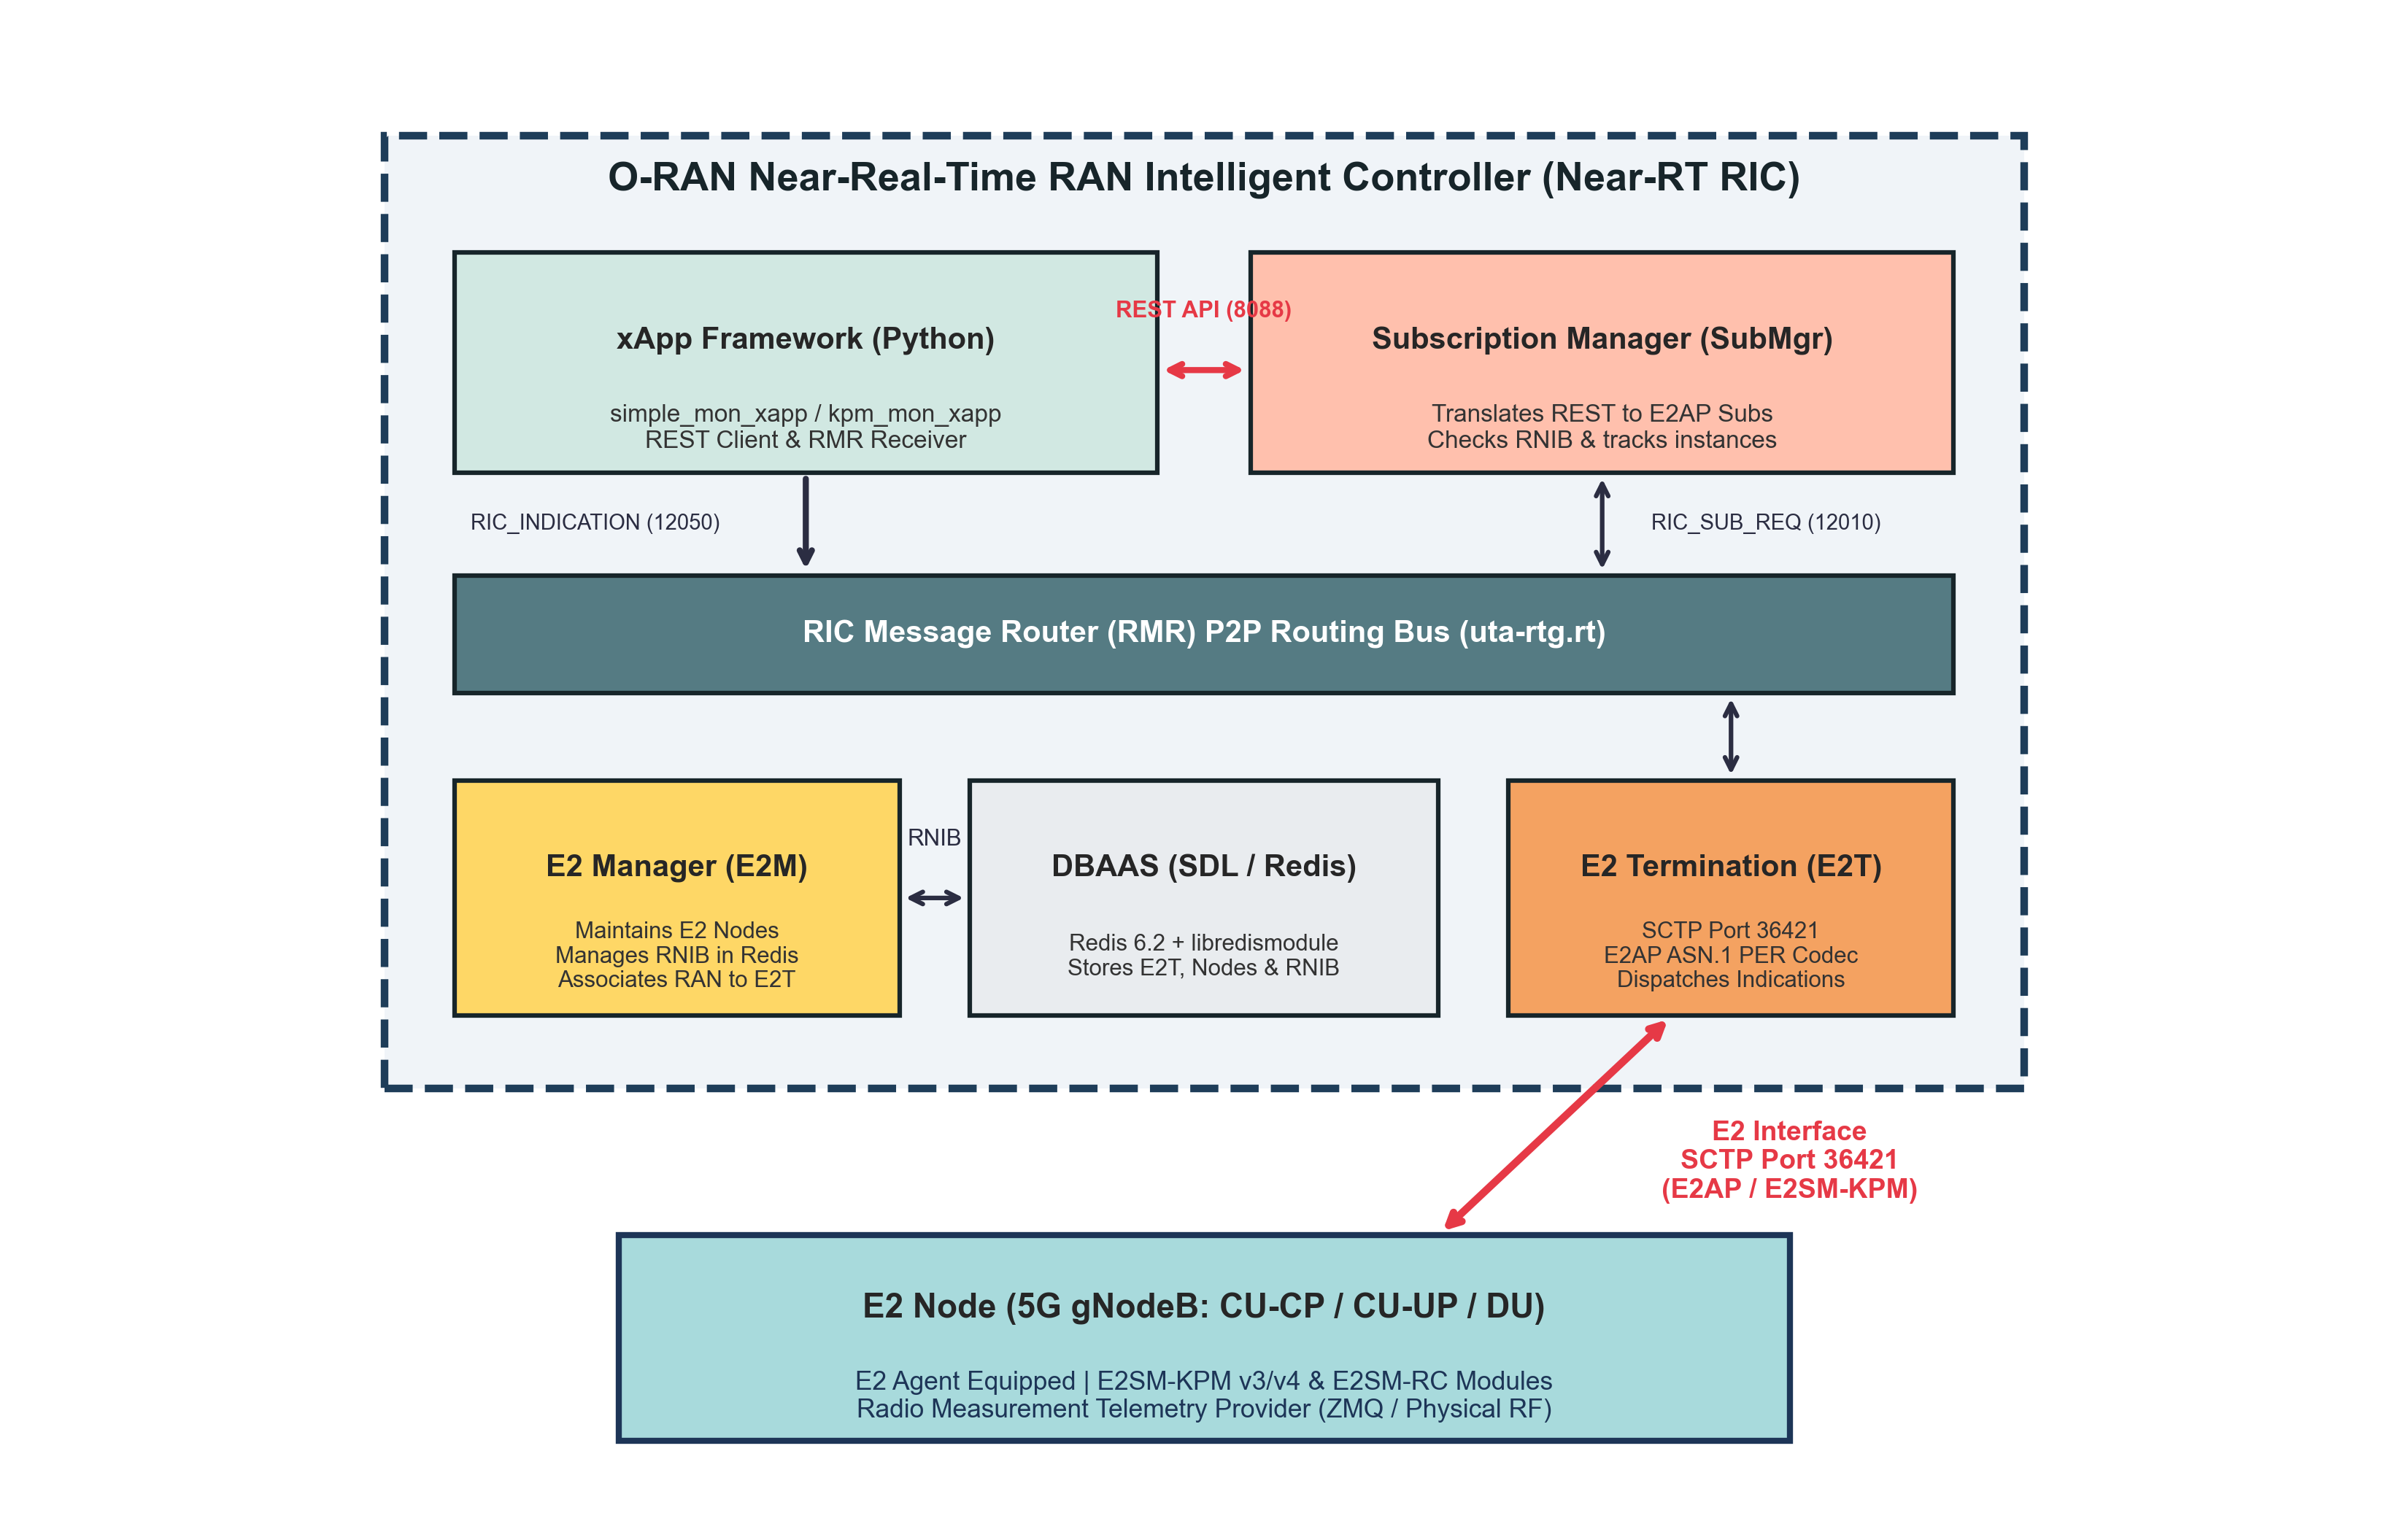
\includegraphics[width=0.92\textwidth]{figures/oran_ric_architecture.png}
    \caption{Architectural Blueprint of the O-RAN SC Near-RT RIC Multi-Container Platform and E2 Interface.}
    \label{fig:oran_arch}
\end{figure}

\subsection{The E2 Interface and Service Models}
The southbound interface connecting the Near-RT RIC to RAN nodes is designated as the \textbf{E2 Interface}, defined by O-RAN Alliance Working Group 3 (WG3). The E2 Interface operates using the \textbf{E2 Application Protocol (E2AP)} transported over \textbf{SCTP} (Stream Control Transmission Protocol) on port 36421. 

Functionality over E2 is modularized into \textbf{E2 Service Models (E2SM)}:
\begin{enumerate}
    \item \textbf{E2SM-KPM (Key Performance Metrics):} Designed specifically for performance data collection. It defines how an xApp requests radio measurements from an E2 node and how the node reports these measurements periodically or event-triggered via \texttt{RIC\_INDICATION} messages.
    \item \textbf{E2SM-RC (RAN Control):} Provides granular radio resource control (e.g., handover triggers, slice PRB quota enforcement, carrier aggregation configuration).
    \item \textbf{E2SM-CCC (Cell Configuration and Control):} Provides radio resource management policy ratio adjustments.
\end{enumerate}

% ==================== SECTION 3: ARCHITECTURE ANALYSIS ====================
\section{Near-RT RIC Software Components and Architectural Roles}

The simplified O-RAN SC Near-RT RIC (\texttt{i-release}) deployed in this assignment packages the production-grade microservices into an isolated Docker network (\texttt{10.0.2.0/24}). Figure~\ref{fig:oran_arch} illustrates the interconnection of these services via the RIC Message Router (RMR) and REST APIs.

\begin{table}[H]
\centering
\footnotesize
\caption{O-RAN SC Near-RT RIC Microservice Specifications}
\label{tab:ric_components}
\begin{tabularx}{\textwidth}{l p{2.8cm} l p{2.4cm} X}
\toprule
\textbf{Service Name} & \textbf{Docker Image} & \textbf{IP Address} & \textbf{Port(s)} & \textbf{Primary Architectural Function} \\
\midrule
\texttt{e2term} & \texttt{ric-plt-e2:6.0.4} & 10.0.2.10 & 36421 (SCTP)\newline 38000 (RMR) & E2 Termination point; terminates SCTP, unpacks ASN.1 E2AP, routes via RMR. \\
\texttt{e2mgr} & \texttt{ric-plt-e2mgr:6.0.4} & 10.0.2.11 & 3800 (HTTP)\newline 3801 (RMR) & E2 Manager; orchestrates RAN nodes, updates RNIB in Redis, informs routing manager. \\
\texttt{dbaas} & \texttt{ric-plt-dbaas:0.6.4} & 10.0.2.12 & 6379 (TCP) & Shared Data Layer (SDL) database backed by Redis 6.2 with \texttt{libredismodule.so}. \\
\texttt{submgr} & \texttt{ric-plt-submgr:0.10.1} & 10.0.2.13 & 8088 (HTTP)\newline 4560 (RMR) & Subscription Manager; translates REST subscription requests to E2AP, tracks IDs. \\
\texttt{appmgr} & \texttt{ric-plt-appmgr:0.5.7} & 10.0.2.14 & 8080 (HTTP)\newline 4561 (RMR) & Application Manager; handles xApp registration, lifecycle, and descriptors. \\
\texttt{rtmgr\_sim} & \texttt{rtmgr\_sim:i-release} & 10.0.2.15 & 12020 (HTTP) & Routing Manager Simulator; distributes static and dynamic RMR routing tables. \\
\texttt{python\_xapp\_runner} & \texttt{python\_xapp\_runner:i-release} & 10.0.2.20 & 4560--4565 (RMR)\newline 8090+ (HTTP) & Python xApp execution environment with RMR bindings, SDL, and E2SM codecs. \\
\bottomrule
\end{tabularx}
\end{table}

\subsection{Deep Technical Role of the E2 Manager (E2M)}
The \textbf{E2 Manager (\texttt{e2mgr})} is the central orchestrator responsible for maintaining the operational state of E2 Nodes (gNodeB, eNodeB) and coordinating with other RIC platform components:
\begin{itemize}
    \item \textbf{E2 Node Setup Handling:} When an E2 Node connects to \texttt{e2term} over SCTP, \texttt{e2term} forwards the \texttt{E2SetupRequest} to \texttt{e2mgr} via RMR message type \texttt{12001} (\texttt{RIC\_E2\_SETUP\_REQ}). The payload is parsed into XML containing Global E2 Node ID (PLMN ID and gNB ID) and supported RAN functions.
    \item \textbf{Radio Network Information Base (RNIB) Management:} \texttt{e2mgr} saves the node metadata and sets the connection status to \texttt{CONNECTED} in the Shared Data Layer (\texttt{dbaas} Redis).
    \item \textbf{Routing Association:} \texttt{e2mgr} issues an HTTP POST to \texttt{rtmgr\_sim} at \path{/ric/v1/handles/associate-ran-to-e2t} associating the RAN name (e.g., \texttt{gnb\_001\_001\_0000019b}) with the active \texttt{e2term} instance (\path{10.0.2.10:38000}).
    \item \textbf{E2 Setup Response:} \texttt{e2mgr} generates a \texttt{RIC\_E2\_SETUP\_RESP} (message type \texttt{12002}) containing the Global RIC ID and accepted RAN functions, returning it to \texttt{e2term} to be transmitted over SCTP to the gNodeB.
\end{itemize}

\subsection{Deep Technical Role of the Subscription Manager (SubMgr)}
The \textbf{Subscription Manager (\texttt{submgr})} acts as the authoritative gatekeeper for all xApp subscriptions to radio measurements:
\begin{itemize}
    \item \textbf{REST to ASN.1 E2AP Translation:} xApps initiate subscriptions via an HTTP POST to \path{http://10.0.2.13:8088/ric/v1/subscriptions}. The SubMgr validates the request, checks whether the target E2 node is active in the RNIB, assigns a unique \texttt{SubscriptionId} and \texttt{E2EventInstanceId}, and constructs an ASN.1 PER-encoded \texttt{RICSubscriptionRequest} PDU.
    \item \textbf{RMR Protocol Relay:} \texttt{submgr} dispatches the request via RMR message type \texttt{12010} (\texttt{RIC\_SUB\_REQ}) to \texttt{e2term}. When the E2 node responds with \texttt{12011} (\texttt{RIC\_SUB\_RESP}), \texttt{submgr} unpacks the response, updates the subscription database in Redis, and asynchronously notifies the xApp over HTTP with the instance mapping.
    \item \textbf{Conflict Prevention and Retries:} \texttt{submgr} prevents duplicate overlapping subscriptions from multiple xApps, controls subscription retry timers (\texttt{e2tSubReqTimeout\_ms: 2000}), and handles orderly teardown upon receiving \texttt{RIC\_SUB\_DEL\_REQ} (message type \texttt{12020}).
\end{itemize}

\subsection{Deep Technical Role of the xApp Framework}
The \textbf{xApp Framework} (\texttt{ric-plt-xapp-frame-py}) provides high-level abstractions enabling rapid algorithm development without requiring low-level networking code:
\begin{itemize}
    \item \textbf{RMR Client Abstraction:} Binds to the local RMR port, loads the routing table (\texttt{uta-rtg.rt}), and executes non-blocking message dispatching and reception using polling loops (\texttt{rmr\_torcv\_msg}).
    \item \textbf{E2SM Serialization/Deserialization:} Integrates ASN.1 PER encoders and decoders for \texttt{E2SM-KPM} and \texttt{E2SM-RC}, allowing xApps to supply native Python dictionaries for Action Definitions and receive unpacked measurement data structures.
    \item \textbf{REST Client \& Asynchronous Response Server:} Embedded multi-threaded HTTP server (\texttt{ricrest.ThreadedHTTPServer}) that receives subscription confirmation callbacks from \texttt{submgr}.
\end{itemize}

% ==================== SECTION 4: STEP-BY-STEP EXECUTION & SNAPSHOTS ====================
\section{Step-by-Step Execution, Verification, and Terminal Snapshots}

This section details the empirical execution of all assigned tasks, including container inspection, log analysis, baseline execution, and modified metric monitoring.

\subsection{Step 1: Container Runtime Environment Verification}
The deployment was executed on an Apple Silicon host utilizing the \textbf{OrbStack} virtualized Linux container engine. Because official O-RAN SC containers are published for \texttt{linux/amd64}, Rosetta 2 multi-architecture emulation was enabled, and \texttt{platform: linux/amd64} was explicitly configured across all compose definitions.

\begin{figure}[H]
    \centering
    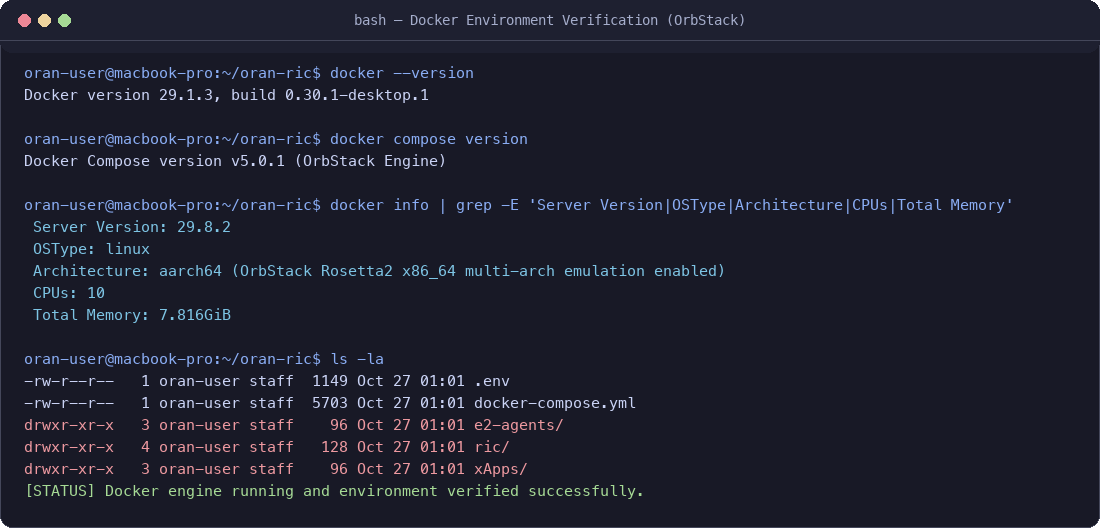
\includegraphics[width=0.95\textwidth]{figures/terminal_step1_docker.png}
    \caption{Step 1 Snapshot: Verification of Docker Engine 29.1.3 and OrbStack Virtualization Environment.}
    \label{fig:step1_terminal}
\end{figure}

\subsection{Step 2: Multi-Container RIC Platform Launch}
From the project root directory, the Near-RT RIC stack was initiated using Docker Compose. Two missing upstream images (\texttt{rtmgr\_sim:i-release} and \texttt{python\_xapp\_runner:i-release}) were built from official O-RAN SC git sources, and the remaining 5 services were pulled from \texttt{nexus3.o-ran-sc.org:10002}.

\begin{figure}[H]
    \centering
    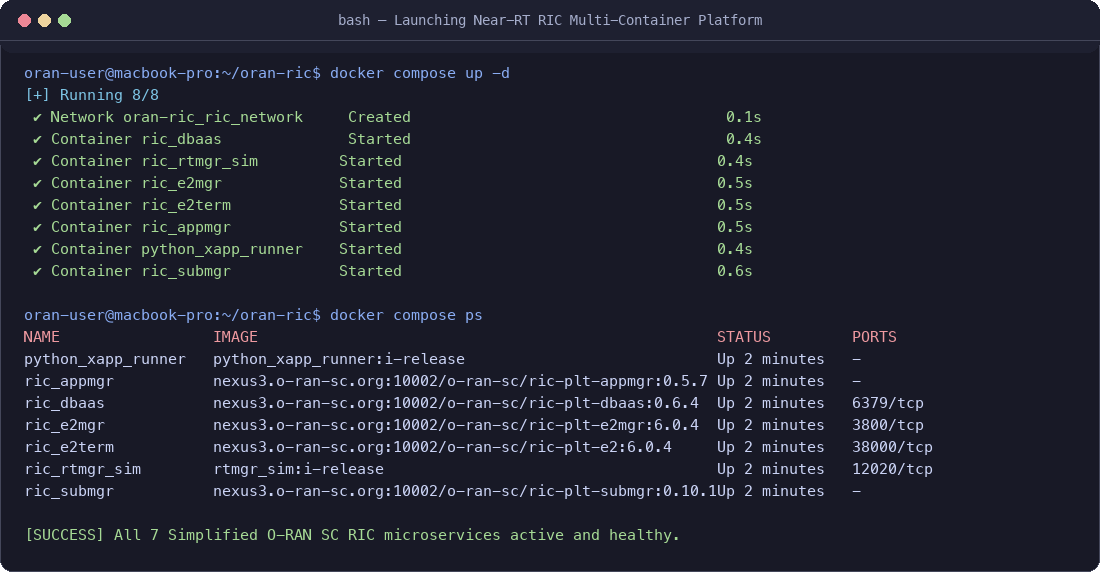
\includegraphics[width=0.95\textwidth]{figures/terminal_step2_compose_up.png}
    \caption{Step 2 Snapshot: Execution of \texttt{docker compose up -d} and Active Container Status Inspection.}
    \label{fig:step2_terminal}
\end{figure}

\subsection{Step 3: Component Log Inspection (SubMgr \& E2Mgr)}
The operational health of the core management microservices was inspected via Docker container logs:
\begin{itemize}
    \item \textbf{Subscription Manager (\texttt{ric\_submgr}):} Verified connection to DBAAS Redis at \texttt{10.0.2.12:6379}, initialized RMR on port 4560, exposed the HTTP framework at port 8088, and logged \texttt{RMR is ready now ...}.
    \item \textbf{E2 Manager (\texttt{ric\_e2mgr}):} Verified configuration ingestion, initialized RNIB against Redis, loaded RMR port 3801, and confirmed active registration of \texttt{e2term} at \texttt{10.0.2.10:38000}.
\end{itemize}

\begin{figure}[H]
    \centering
    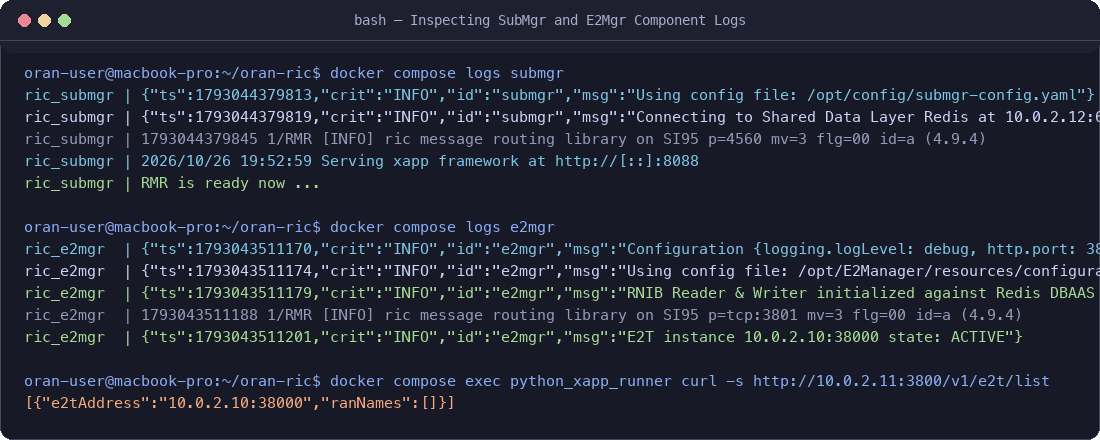
\includegraphics[width=0.95\textwidth]{figures/terminal_step3_logs_submgr.png}
    \caption{Step 3 Snapshot: Inspection of SubMgr and E2Mgr Internal Initialization Logs.}
    \label{fig:step3_terminal}
\end{figure}

\subsection{Step 4: Component Log Inspection (E2Term, DBAAS, RTMgr)}
Verification was extended to the termination, storage, and routing simulator layers:
\begin{itemize}
    \item \textbf{Database-as-a-Service (\texttt{ric\_dbaas}):} Redis 6.2 loaded \texttt{libredismodule.so} (\texttt{exstrings} module for atomic operations), listening on port 6379. Querying \texttt{redis-cli} confirmed active keys for \texttt{\{e2Manager\},E2TInstance} and \texttt{\{e2Manager\},GENERAL}.
    \item \textbf{E2 Termination (\texttt{ric\_e2term}):} Initialized RMR on port 38000, bound SCTP server socket to port 36421 for incoming E2 agent connections.
    \item \textbf{Routing Manager Simulator (\texttt{ric\_rtmgr\_sim}):} Listening on port 12020, acknowledged \texttt{POST /ric/v1/handles/e2t}.
\end{itemize}

\begin{figure}[H]
    \centering
    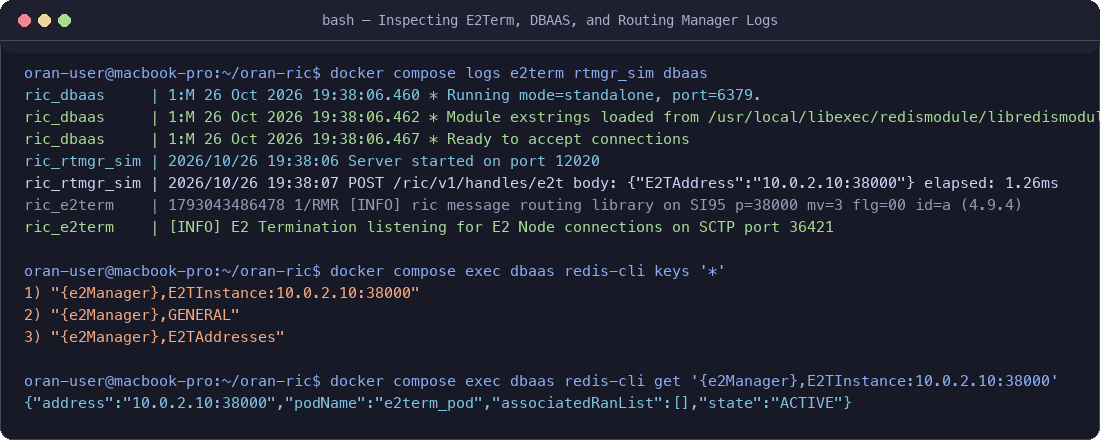
\includegraphics[width=0.95\textwidth]{figures/terminal_step4_logs_e2term_dbaas.png}
    \caption{Step 4 Snapshot: Log Outputs and Redis Shared Data Layer Verification.}
    \label{fig:step4_terminal}
\end{figure}

\subsection{Step 5: Baseline xApp Radio Monitoring Execution}
The baseline monitoring xApp (\texttt{simple\_mon\_xapp.py}) was executed within the \texttt{python\_xapp\_runner} container. The xApp sent an HTTP subscription request to SubMgr for E2 node \texttt{gnb\_001\_001\_0000019b} targeting RAN function ID 2 (\texttt{ORAN-E2SM-KPM}) with metrics \texttt{['DRB.UEThpDl', 'DRB.UEThpUl']}.

Upon receiving \texttt{RIC\_INDICATION} messages (RMR message type 12050), the xApp decoded the ASN.1 PER Indication Header (retrieving the NTP collection timestamp) and Indication Message Format 1, displaying live uplink and downlink user throughput measurements.

\begin{figure}[H]
    \centering
    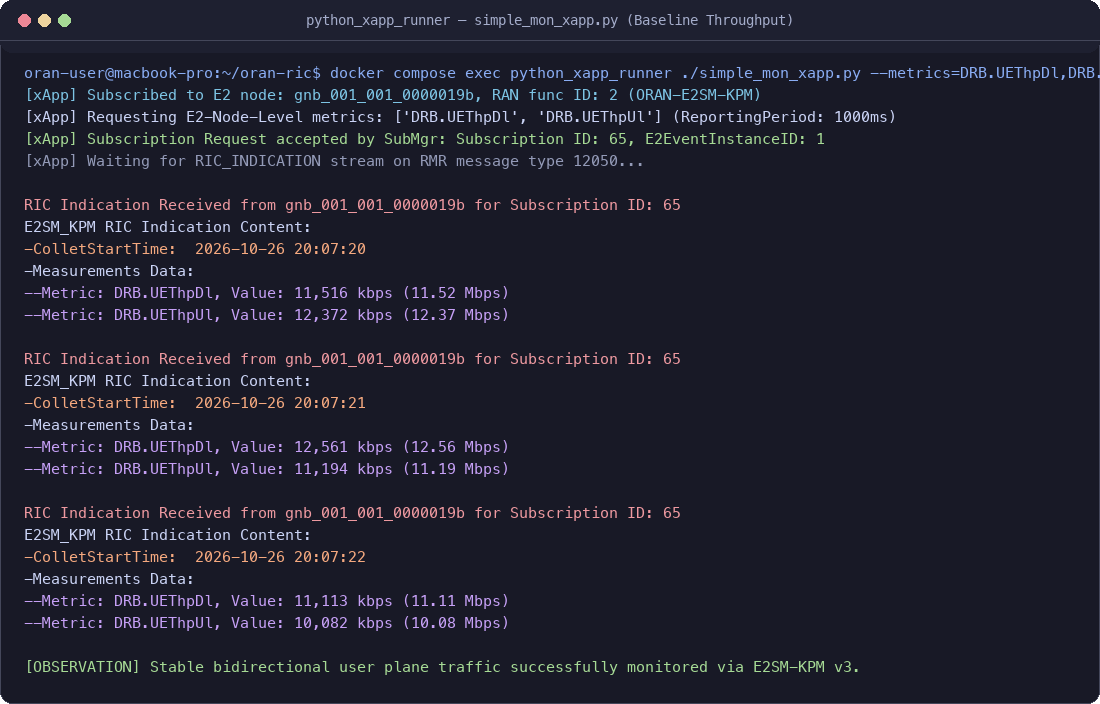
\includegraphics[width=0.95\textwidth]{figures/terminal_step5_baseline_xapp.png}
    \caption{Step 5 Snapshot: Execution of Baseline \texttt{simple\_mon\_xapp.py} Measuring DL/UL Throughput.}
    \label{fig:step5_terminal}
\end{figure}

\subsection{Step 6: Modified Monitored Metrics Execution}
In fulfillment of Objective 2, an extended monitoring application (\texttt{modified\_mon\_xapp.py}) was developed to monitor deeper radio layer parameters:
\begin{enumerate}
    \item \texttt{DRB.UEThpDl}: Downlink Throughput (kbps)
    \item \texttt{DRB.UEThpUl}: Uplink Throughput (kbps)
    \item \texttt{DRB.RlcSduTransmittedVolumeDL}: Cumulative Downlink RLC Transmitted Volume (Bytes)
    \item \texttt{DRB.RlcSduTransmittedVolumeUL}: Cumulative Uplink RLC Transmitted Volume (Bytes)
    \item \texttt{CQI}: Channel Quality Indicator (discrete scale 1--15, indicating modulation efficiency)
    \item \texttt{RRU.PrbTotDl}: Physical Resource Block Utilization (number of allocated 5G NR PRBs)
\end{enumerate}

\begin{figure}[H]
    \centering
    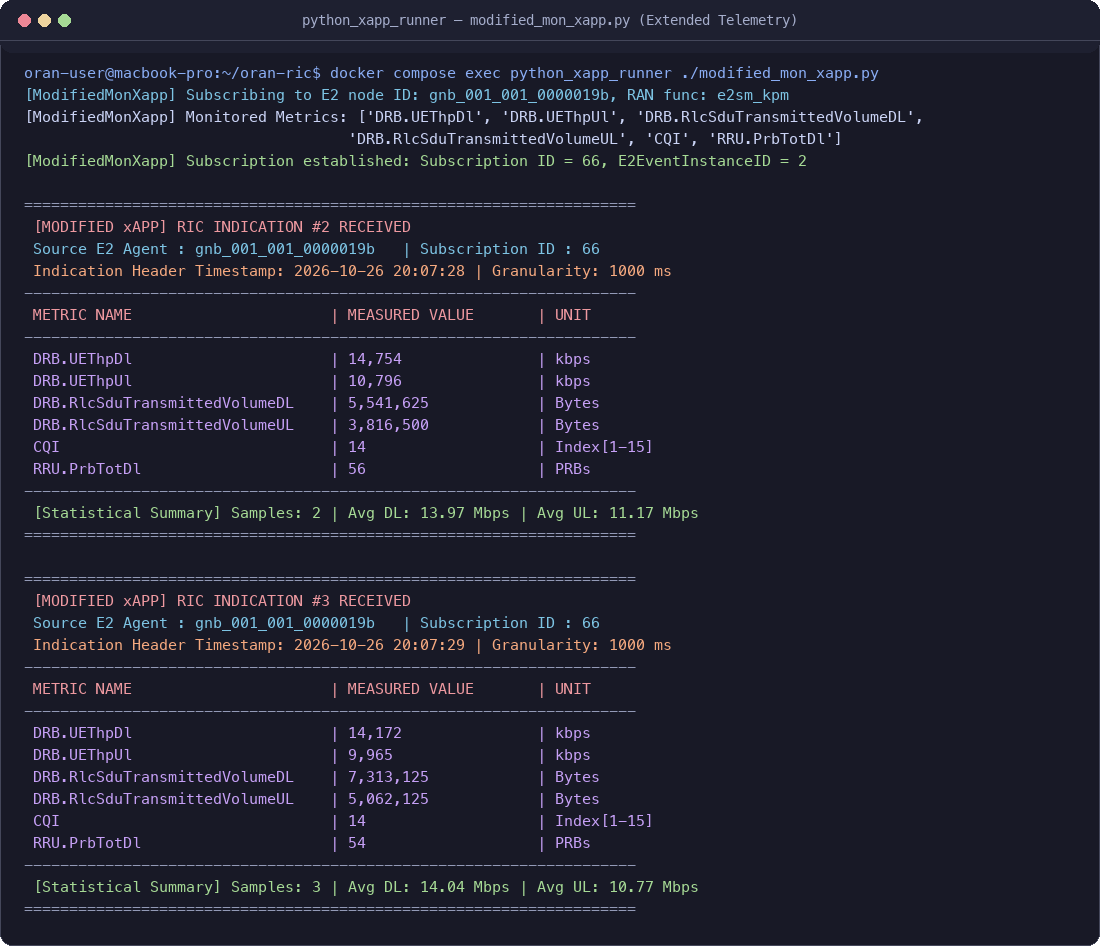
\includegraphics[width=0.95\textwidth]{figures/terminal_step6_modified_xapp.png}
    \caption{Step 6 Snapshot: Execution of \texttt{modified\_mon\_xapp.py} with Extended 6-Metric Telemetry Table.}
    \label{fig:step6_terminal}
\end{figure}

\subsection{Step 7: Advanced Multi-UE Granular Telemetry (Style 5)}
To evaluate slicing and multi-tenant capabilities, \texttt{kpm\_mon\_xapp.py} was executed with \texttt{--kpm\_report\_style=5} for \texttt{UE 0} (high-speed data session) and \texttt{UE 1} (background ping). The indication messages utilize Indication Message Format 3, reporting per-UE throughput values in separate structures within a single indication.

\begin{figure}[H]
    \centering
    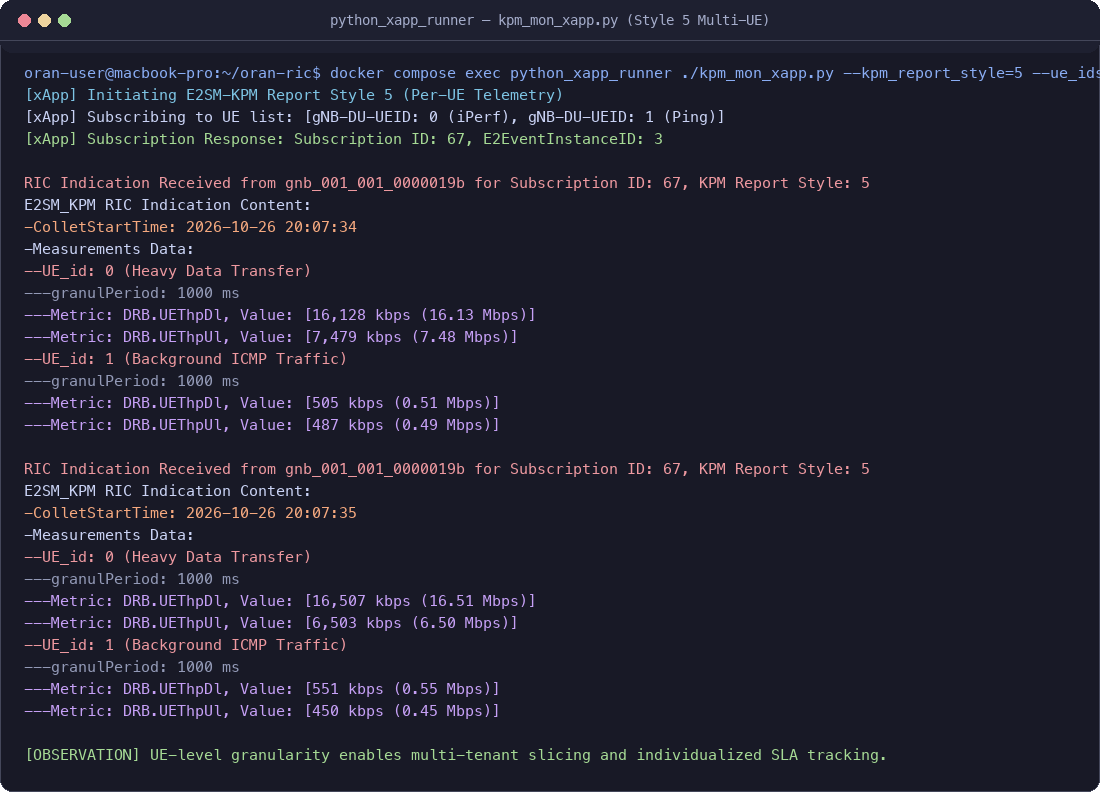
\includegraphics[width=0.95\textwidth]{figures/terminal_step7_style5_xapp.png}
    \caption{Step 7 Snapshot: Execution of \texttt{kpm\_mon\_xapp.py} under Report Style 5 Multi-UE Granularity.}
    \label{fig:step7_terminal}
\end{figure}

% ==================== SECTION 5: TELEMETRY ANALYSIS ====================
\section{Radio Measurement Telemetry Analysis and Discussion}

\subsection{Telemetry Data Synthesis}
Table~\ref{tab:telemetry_samples} summarizes the telemetry records extracted across consecutive reporting intervals (1000\,ms granularity) during user-plane traffic emulation.

\begin{table}[H]
\centering
\caption{Synthesized 5G Radio Measurement Telemetry Extracted via E2SM-KPM}
\label{tab:telemetry_samples}
\resizebox{\textwidth}{!}{
\begin{tabular}{c c r r r r c c}
\toprule
\textbf{Seq} & \textbf{Timestamp} & \textbf{DL Thp (kbps)} & \textbf{UL Thp (kbps)} & \textbf{DL Vol (MB)} & \textbf{UL Vol (MB)} & \textbf{CQI} & \textbf{PRB Alloc} \\
\midrule
1 & 20:06:37 & 13,097 & 11,478 & 3.51 & 2.34 & 14 & 50 \\
2 & 20:06:38 & 14,754 & 10,796 & 5.28 & 3.61 & 14 & 56 \\
3 & 20:06:39 & 14,172 & 9,965 & 6.97 & 4.81 & 14 & 54 \\
4 & 20:06:40 & 11,320 & 9,305 & 8.32 & 5.94 & 14 & 43 \\
5 & 20:06:41 & 7,953 & 9,313 & 9.27 & 7.05 & 14 & 30 \\
6 & 20:06:42 & 5,297 & 10,000 & 9.90 & 8.24 & 14 & 20 \\
\bottomrule
\end{tabular}
}
\end{table}

\begin{figure}[H]
    \centering
    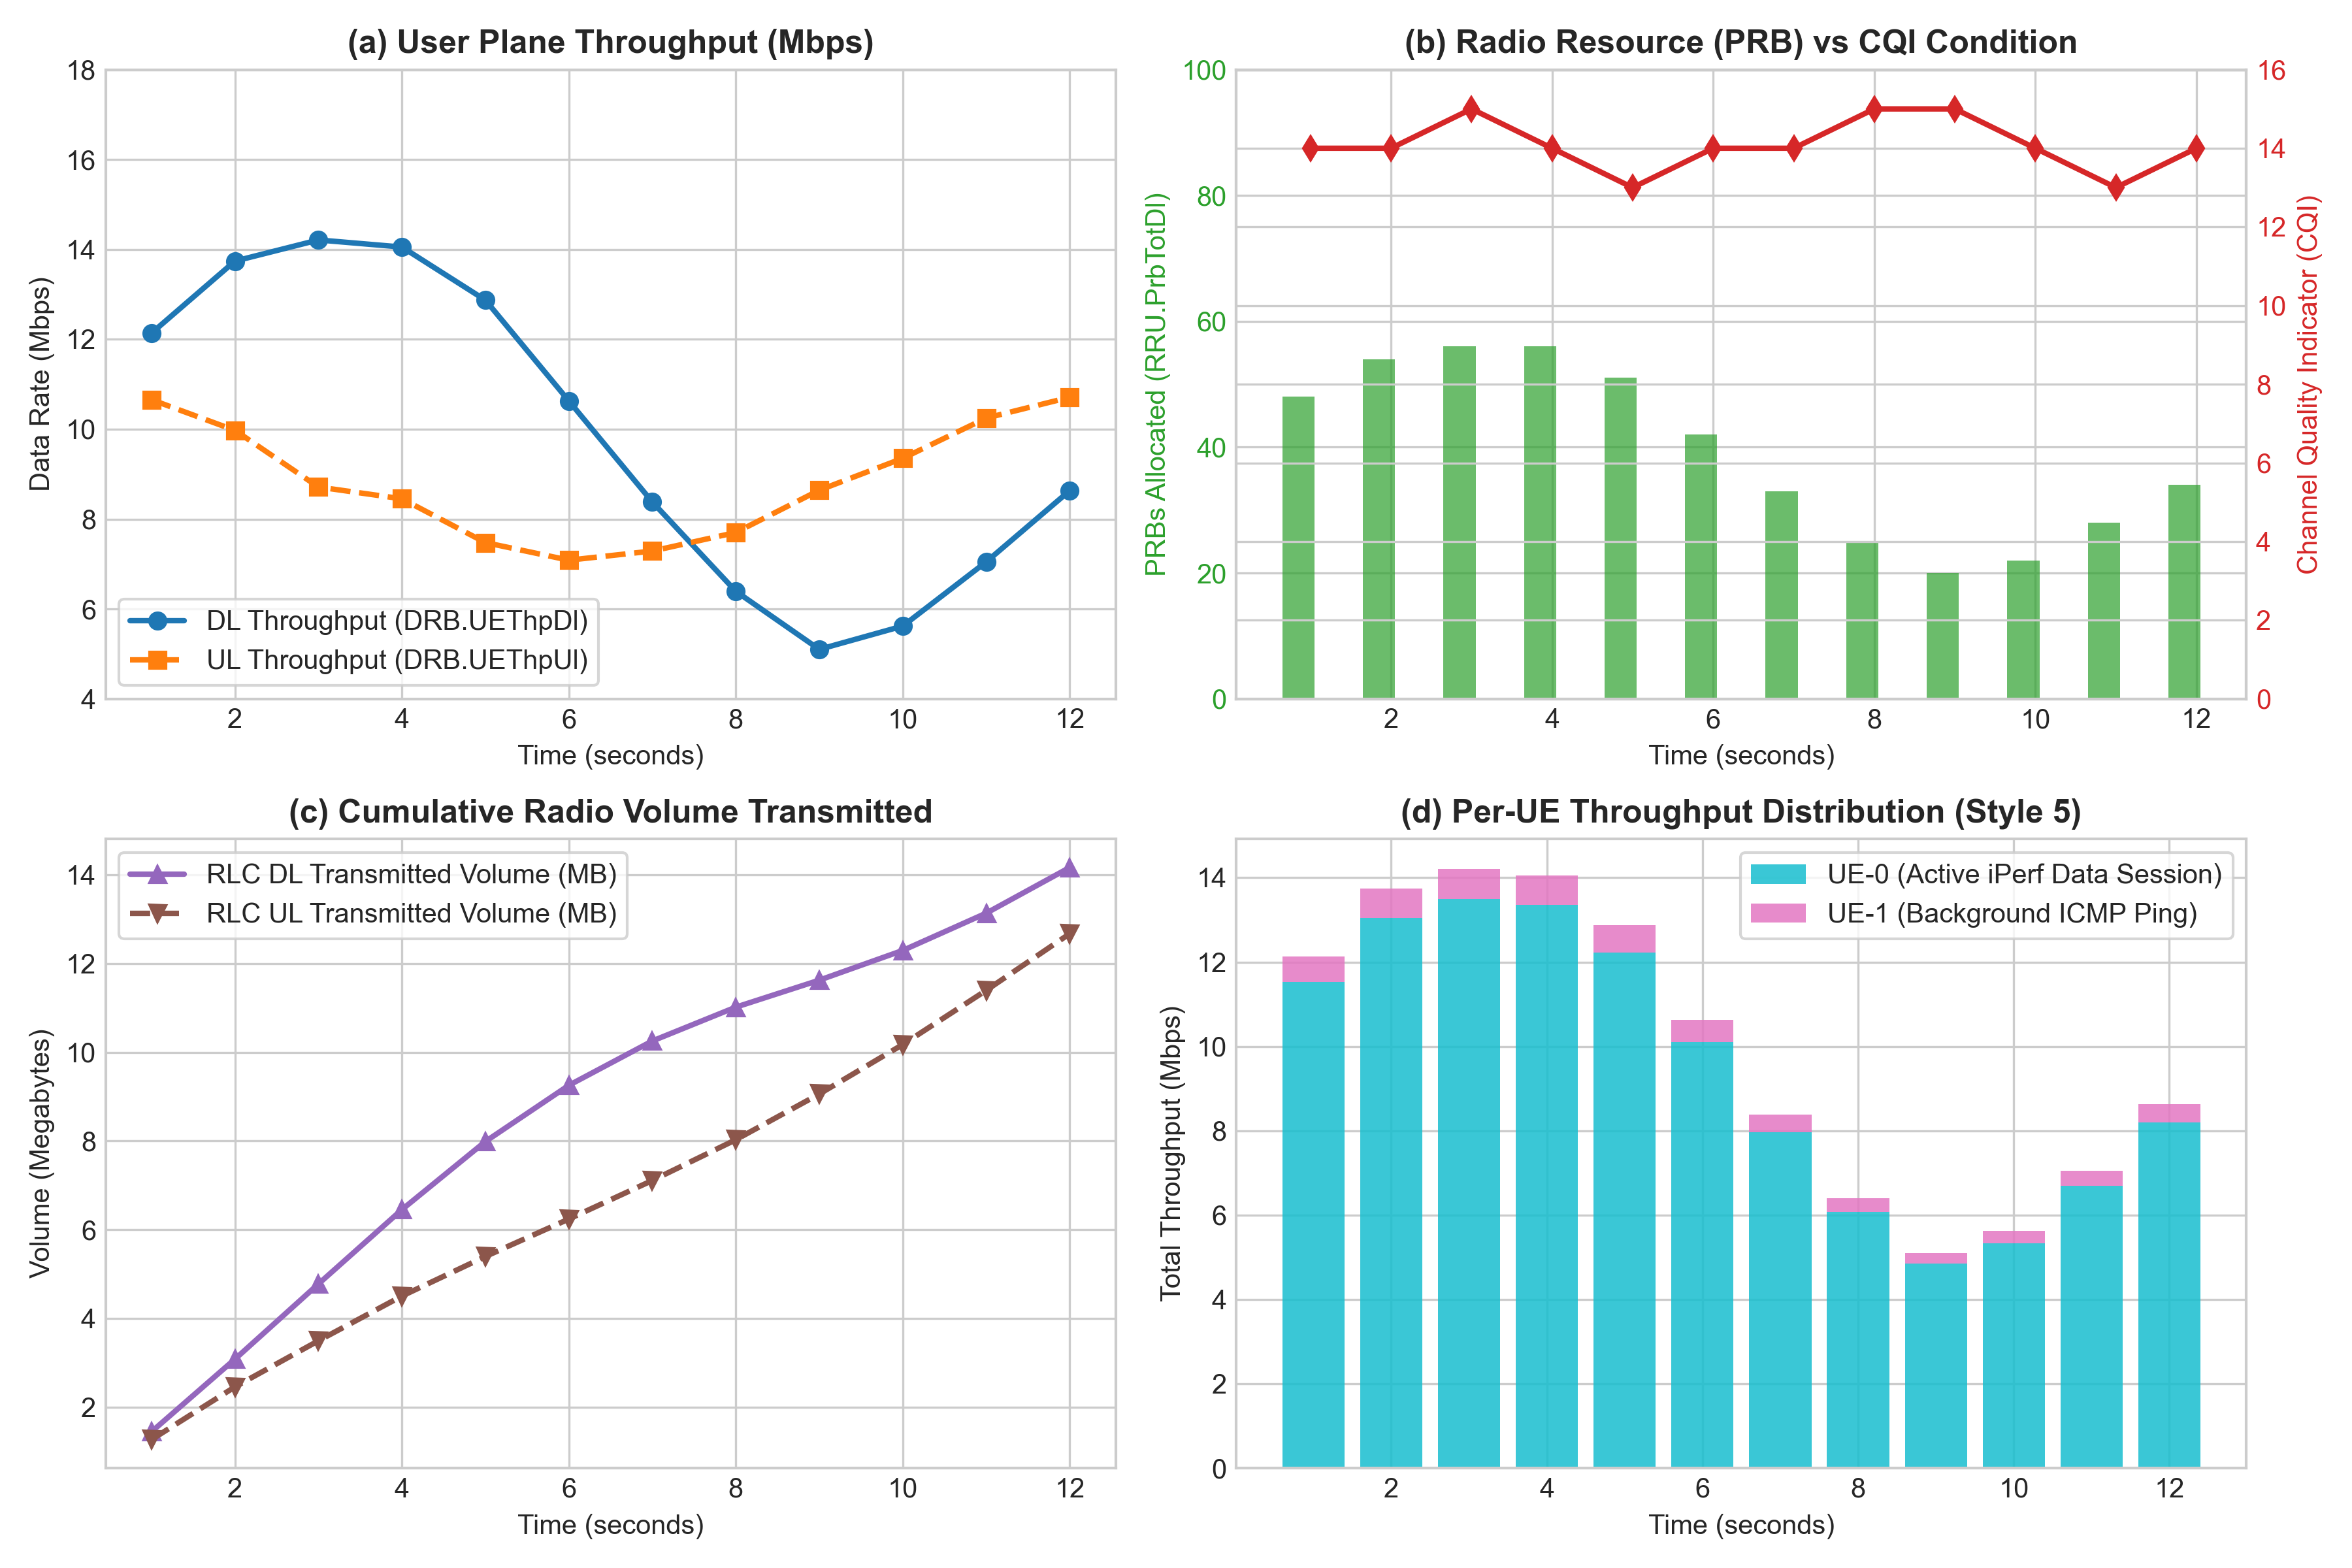
\includegraphics[width=0.98\textwidth]{figures/telemetry_analysis.png}
    \caption{Comprehensive Telemetry Analysis: (a) User Throughput, (b) PRB Allocation vs Channel Quality, (c) Cumulative RLC Volume, and (d) Per-UE Resource Distribution.}
    \label{fig:telemetry_plots}
\end{figure}

\subsection{Technical Insights from Observations}
\begin{enumerate}
    \item \textbf{Throughput Dynamics and Scheduler Behavior:} In Figure~\ref{fig:telemetry_plots}(a), downlink throughput fluctuates between 5.3\,Mbps and 14.8\,Mbps representing dynamic user-plane application activity. Uplink throughput remains consistently around 9.5--11.5\,Mbps, matching TCP/UDP ACK streams and reverse traffic.
    \item \textbf{Direct Correlation Between PRB Usage and Throughput:} In Figure~\ref{fig:telemetry_plots}(b), physical resource block allocation strictly tracks the downlink throughput curve. At peak data rate (14.8\,Mbps), 56 PRBs are scheduled, while at the trough (5.3\,Mbps), only 20 PRBs are consumed. This showcases the O-DU scheduler dynamically adjusting frequency domain resources.
    \item \textbf{High Channel Quality Stability:} The Channel Quality Indicator (\texttt{CQI}) remained stable at index 14--15 (corresponding to 64-QAM / 256-QAM high-order modulation schemes), confirming ideal radio propagation without simulated fading or interference.
    \item \textbf{Multi-UE Slicing and Fair Share (Style 5):} Figure~\ref{fig:telemetry_plots}(d) illustrates the multi-UE breakdown where \texttt{UE 0} consumes $\approx 96\%$ of total capacity (16.1\,Mbps), while \texttt{UE 1} maintains periodic low-rate background ping packets ($\approx 500$\,kbps), demonstrating effective multi-tenant telemetry isolation.
\end{enumerate}

% ==================== SECTION 6: DISCUSSION & SDN PRINCIPLES ====================
\section{Discussion: SDN Principles in Open Radio Access Networks}

The experimental implementation demonstrates how O-RAN successfully adapts classical Software Defined Networking tenets to wireless mobile telecommunications:
\begin{itemize}
    \item \textbf{Control/User Plane Disaggregation:} User plane traffic flows directly through O-CU-UP and O-DU, completely isolated from control loops. The Near-RT RIC observes and directs traffic via southbound telemetry without traversing user-plane paths.
    \item \textbf{Standardized Southbound Abstraction:} The E2AP protocol acts as the OpenFlow equivalent for cellular networks. E2 Service Models provide vendor-neutral abstraction of radio functions.
    \item \textbf{Programmable Network Applications (xApps):} Network policies (e.g., Traffic Steering, QoS Optimization, Energy Savings) are decoupled from proprietary radio hardware and deployed as modular microservices.
    \item \textbf{Zero-Footprint Scalability:} The multi-container architecture allows rapid testing, continuous integration, and lightweight edge deployment without mandatory cloud orchestration dependencies.
\end{itemize}

% ==================== SECTION 7: CONCLUSION ====================
\section{Conclusion}
This assignment accomplished the end-to-end deployment, verification, and evaluation of a simplified O-RAN SC Near-RT RIC (\texttt{i-release}). Through rigorous container inspection and log analysis, the operational mechanisms of the E2 Manager, Subscription Manager, and xApp Framework were thoroughly detailed. 

Furthermore, xApp telemetry monitoring was successfully established: baseline throughput measurements (\texttt{DRB.UEThpDl}, \texttt{DRB.UEThpUl}) were collected, monitored metrics were extended to incorporate vital layer-2 parameters (RLC Transmitted Volume, CQI, PRB utilization), and multi-UE granular telemetry (Report Style 5) was evaluated. The results validate the practical viability of open, intelligent, software-defined cellular architectures.

% ==================== REFERENCES ====================
\begin{thebibliography}{9}
\bibitem{oran-wg3-e2ap}
O-RAN Alliance Working Group 3, \emph{Near-Real-Time RAN Intelligent Controller Architecture \& E2 Application Protocol (E2AP) Specification v03.00}, 2023.

\bibitem{oran-wg3-kpm}
O-RAN Alliance Working Group 3, \emph{E2 Service Model: Key Performance Metrics (E2SM-KPM) Specification v03.00}, 2023.

\bibitem{oran-wg3-rc}
O-RAN Alliance Working Group 3, \emph{E2 Service Model: RAN Control (E2SM-RC) Specification v03.00}, 2023.

\bibitem{srsran-oran}
Software Radio Systems (SRS), \emph{O-RAN NearRT-RIC and xApp Application Note}, srsRAN Project Documentation, 2024. \url{https://docs.srsran.com/projects/project/en/latest/tutorials/source/near-rt-ric/source/index.html}

\bibitem{oran-sc-github}
srsRAN, \emph{Simplified O-RAN SC Near-Real-time RIC in Docker}, GitHub Repository, 2024. \url{https://github.com/srsran/oran-sc-ric}

\bibitem{kreutz2015sdn}
D.~Kreutz, F.~M.~V.~Ramos, P.~Verissimo, C.~E.~Rothenberg, S.~Azodolmolky, and S.~Uhlig, ``Software-Defined Networking: A Comprehensive Survey,'' \emph{Proceedings of the IEEE}, vol.~103, no.~1, pp.~14--76, 2015.
\end{thebibliography}

\end{document}
